% !TeX spellcheck=en_GB
\documentclass[a4paper]{article}

\usepackage{geometry}
\usepackage{fullpage}
\usepackage{todonotes}
\usepackage{float}
\usepackage{graphicx}
\usepackage{subcaption}
\usepackage{hyperref}
\usepackage{amsmath}

\newcommand{\newpar}{\bigskip\noindent}

\author{Mikael Lindemann (bjm466@alumni.ku.dk)}
\title{Lecture Notes - Approximation Algorithms}

\begin{document}
	\maketitle
	\noindent An approximation algorithm is an algorithm that returns a near-optimal solutions in polynomial time. Near-optimal is defined by an \textit{approximation ratio}, $\rho(n)$. If $C^*$ denotes the value of an optimal solution and $C$ denotes the value of an approximation, then $\rho(n)$ in \autoref{approx:ratio} denotes the approximation ratio, where $n$ denotes the size of the problem.
	
	\begin{equation}\label{approx:ratio}
		max\left(\frac{C}{C^*}, \frac{C^*}{C}\right) \leq \rho(n)
	\end{equation}
	
	\section{Approximation schemes}
	\textbf{Polynomial Time Approximation Scheme (PTAS)}
	
	\noindent Choose an $\varepsilon > 0$. Then a PTAS is a $(1+\varepsilon)$-approximation algorithm for a NP-hard minimization problem, where the running time is bounded by a polynomial in the size of the problem instance $I$.
	
	\newpar \textbf{Fully Polynomial Time Approximation Scheme (FPTAS)}
	
	\noindent Same as PTAS, with the extra requirement that the running time must be bounded in both a polynomial of the instance size, and in $1/\varepsilon$.
	
	\newpar For maximization problems, we should replace $(1+\varepsilon)$ with $(1-\varepsilon)$.
	
	\section{Vertex cover}
	\textbf{Problem:} Choose a subset, $C$, of vertices $V(G)$, such that all edges have one endpoint in $C$.
	
	\subsection{Matching}
	\textbf{Problem:} Find a subset of edges in $G$, such that no two edges share a vertex.\\
	\textbf{Maximal matching:} A matching, such that if another edge was included, it would no longer be a matching.\\
	\textbf{Maximum matching:} The largest possible maximal matching for $G$.
	
	\subsection{Vertex cover and Matching}
	By definition, no vertex can cover more than one edge of a matching. Also the size of every vertex cover, in number of vertices, is at least the size of any matching, in number of edges. A vertex cover can be found by taking any maximal matching, and take all end-vertices of all edges in the matching. Since we choose all vertices in a matching for our vertex cover, we do not want a maximum matching, since this would include event more vertices.

	\noindent\textbf{Maximal matching gives a 2-Approximation for vertex cover}:
	
	\noindent Let $C$ denote the vertex cover obtained from a maximal matching $M$. $|C|$ denotes the number of vertices in $C$. Let $C^*$ denote the optimal vertex cover. $|C^*|$ denotes the number of vertices in $C^*$. Let $|M|$ denote the number of edges in $M$. Since every edge of any matching needs to be covered in vertex cover, we know that $|M|\leq|C^*|$. Since $C$ is obtained by taking all vertices of a matching, we know that $|C| = 2|M|$. Therefore: $|C| = 2|M| \leq 2|C^*|$. By inserting $|C|$ and $2|C^*|$ into \autoref{approx:ratio} we see that the approximation factor is 2.
	
	\begin{figure}[H]
		\centering
		\begin{subfigure}[t]{.45\textwidth}
			\centering
			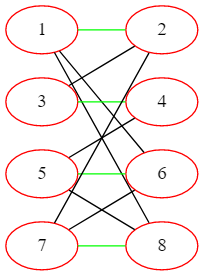
\includegraphics[scale=.5]{figures/bipartite-matching.png} 
			\caption{In this example, our approximation will find a vertex cover of size 8, which is exactly a factor of two away from the optimal, which in this example could be to pick all odd-numbered vertices.}
		\end{subfigure}
		~
		\begin{subfigure}[t]{.45\textwidth}
			\centering
			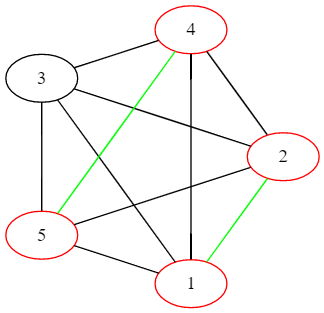
\includegraphics[scale=.5]{figures/5fullyconnected-matching.png}
			\caption{In this example, our approximation will find the optimal vertex cover of size 4.}
		\end{subfigure}
	\caption{Examples of found matchings and vertex covers. The green edges are the chosen edges for a maximal matching, and the red vertices denote the vertex cover found by using the matching.}
	\label{vertexcover:examples}
	\end{figure}

	\noindent In \autoref{vertexcover:examples} we see that in some cases, the approximation will find an optimal solution, while in other cases, it can find solutions that are a factor of 2 away from being optimal. This is in line with the argument shown above.
	
	\subsection{Weighted Vertex Cover}
	In weighted vertex cover, each vertex $i$ has an associated weight $w_i$. We want to find the set of vertices that covers all edges, while minimizing the weight of the chosen vertices. In \autoref{wvc} an ILP and LP relaxation is given for the weighted vertex cover problem.
	
	\begin{figure}[H]
		\begin{subfigure}{.45\textwidth}
			\begin{alignat*}{4}
				& \text{minimize} & \sum_{i\in V}w_ix_i & &\\
				& \text{subject to} \quad & x_i + x_j & \geq 1 && \forall_{(i,j) \in E}\\
				& & x_i & \in \{ 0, 1 \} \quad && \forall_{i \in V}
			\end{alignat*}
			\caption{}
			\label{wvc:ilp}
		\end{subfigure}
		~
		\begin{subfigure}{.45\textwidth}
			\begin{alignat*}{4}
				& \text{minimize} & \sum_{i\in V}w_ix_i &\\
				& \text{subject to} \quad & x_i + x_j & \geq 1 && \forall_{(i,j) \in E}\\
				& & x_i & \geq 0 \quad && \forall_{i \in V}
			\end{alignat*}
			\caption{}
			\label{wvc:lp}
		\end{subfigure}
		\caption{The Weighted Vertex Cover problem as Integer Linear Programming (a) and the Linear Programming Relaxation (b).}
		\label{wvc}
	\end{figure}
	
	\noindent Let $x^*$ denote the optimal solution to the LP relaxation. We can construct a vertex cover by choosing all vertices with $x^*_i \geq \frac{1}{2}$. From the constraints $x_i + x_j \geq 1$ we can see that this is a vertex cover, since at least one of $x_i$ and $x_j$ must have a value higher than $\frac{1}{2}$.
	
	\noindent In the following $w(S)$ denotes the total weight of the vertices in $S$. Let $S = \{i | x^*_i \geq \frac{1}{2}\}$ denote a vertex cover obtained by this method. Let $S^*$ be an optimum vertex cover. Then $w(S^*) \geq \sum_{i \in V} w_i x^*_i$ because $x^*$ denotes the solution to the LP relaxation. $\sum_{i \in V} w_i x^*_i \geq \sum_{i \in S} w_i x^*_i$ because $S \subseteq V$. $\sum_{i \in S} w_i x^*_i \geq \frac{1}{2}\sum_{i \in S} w_i$ because all vertices $i \in S$ has a value $x_i \geq \frac{1}{2}$. The last step is $\frac{1}{2}\sum_{i \in S} w_i = \frac{1}{2}w(S)$. Putting everything together and we have $w(S^*) \geq \frac{1}{2}w(S)$. This gives an approximation ratio of 2.

	\subsubsection{Pricing method}
	We can also construct the dual of the LP relaxation of the weighted vertex cover problem. This is found in \autoref{wvc:lp:dual}.
	
	\begin{figure}[H]
		\begin{alignat*}{4}
		& \text{maximize} & \sum_{e\in E}\quad y_e & \\
		& \text{subject to} \quad & \sum_{e = (i,j) \in E} y_e & \leq w_i \quad && \forall_{i \in V}\\
		& & y_e & \geq 0 && \forall_{e\in E}
		\end{alignat*}
		\caption{The dual of \autoref{wvc:lp}.}
		\label{wvc:lp:dual}
	\end{figure}
	
	\newpar Looking at the constraints we can see that for all vertices, $i$, the profit of picking an adjacent edge, $e = (i,j)$ is $y_e$. The sum of edges for a vertex, however, cannot exceed $w_i$, that is, the weight, or cost, of including this vertex in the vertex cover. A vertex is said to be tight if its dual constraint has no slack, that is, if we cannot increase any adjacent edge's dual variable.
	
	\noindent The pricing method for vertex cover uses exactly this. In the beginning we set $y_e = 0$ for all edges $e$ in $E$. While there is an edge $e = (i,j)$ such that neither $i$ or $j$ is tight, we increase the value of $y_e$ until one of $i$ or $j$ becomes tight. When no more edges can have their value increased, the vertex cover is all tight vertices.
	
	This method is polynomial, in each iteration, we pick an edge, and increase its value until some vertex goes tight. Therefore at least one vertex is added to the vertex cover in each iteration. Since all edges have at least one tight vertex, all edges are covered by the set of vertices. Also, we can again show that this is a 2-approximation. Let $C$ denote the weighted vertex cover obtained by the pricing method and let $C^*$ denote an optimum weighted vertex cover.
	
	\newpar By definition, the weight of a cover can be written as: $w(C) = \sum_{i\in C}w_i = \sum_{i\in C}\sum_{e = (i,j)}y_e$. Since $C$ is a subset of $V$ and $y_e \geq 0$ for all $e$, $\sum_{i\in C}\sum_{e = (i,j)}y_e \leq \sum_{i \in V}\sum_{e = (i,j)}y_e$. But since we only fix $i$, we are actually summing up each edge twice. This gives us $\sum_{i \in V}\sum_{e = (i,j)}y_e = 2\sum_{e\in E}y_e \leq 2w(C^*)$. The last inequality comes from the definition of the dual problem of the integer linear program. Again, the approximation ratio is two for this problem.
	
	\section{Remaining Topics}
	Since all the included examples have 2-approximations, it might seem intuitive that all NP-hard problems have 2-approximations. This is not the case though. In the lecture we went over the following problems:
	
	\noindent For the \textbf{Metric Travelling Salesman Problem}: In the lecture we were shown a 2-approximation using minimum spanning trees but also a $\frac{3}{2}$-approximation using minimum spanning trees as well as matching over the vertices with odd degree in the MST.
	
	\noindent For the \textbf{Uniform Knapsack Problem} where the weight to profit ratio is always 1, a 2-approximation was shown. The approximation sorts the items by non-increasing volume, takes items as long as there is still room in the knapsack.
	
	\noindent For the \textbf{General Knapsack Problem} we were shown two approximation algorithms. Using the same procedure as above, just sorting by profit-to-volume ratio, we pick elements until we run out of space in the knapsack. This gives a 2-approximation.
	
	\noindent The other approximation solves knapsack using dynamic programming. The original formulation of the dynamic program will solve knapsack to optimality. But since the running time of the algorithm is dependent on $P$ which denotes the largest possible profit, the running time might be longer than the amount of time that we can weight. Therefore we apply scaling, that is, we divide the profits and volumes by a number, $K$, and round down if necessary. This reduces the running time, but might introduce errors into the result, since we can no longer distinguish close values. By setting $K = \varepsilon P/n$ where $n$ is the number of items, we can create a $(1+\varepsilon)$-approximation. This makes it possible for us to vary $\varepsilon$ in order to prioritize between fast but inaccurate solutions, or slow but more precise solutions. The time complexity was shown to be polynomial in both $n$ and $\frac{1}{\varepsilon}$ and therefore this approximation algorithm is FPTAS.
	
\end{document}